\chapter{Application to a Heuristic Algorithm for Travelling Salesman}

In this section we are going to present an application of the Azuma-Hoeffding inequality to prove the convergence to the mean of a linear approximation algorithm for the \textit{Travelling Salesman Problem}. 

\section*{The Algorithm}

Let $X_1,\ldots, X_N$ be a sample of $N$ uniformly distributed points in a compact square $[0,L]\times [0,L]$. The algorithm divides this square in $M$ stripes of width $L/M$ each. Then, it connects each of the points in each of the stripes vertically and connects the top-most of one stripe with the top-most of the next one (or viceversa as the image below shows).

\begin{figure}[h]\label{TSP:pic0}
    \centering
    \subfloat[Uniform sample]{\label{TSP:pic0.1}
        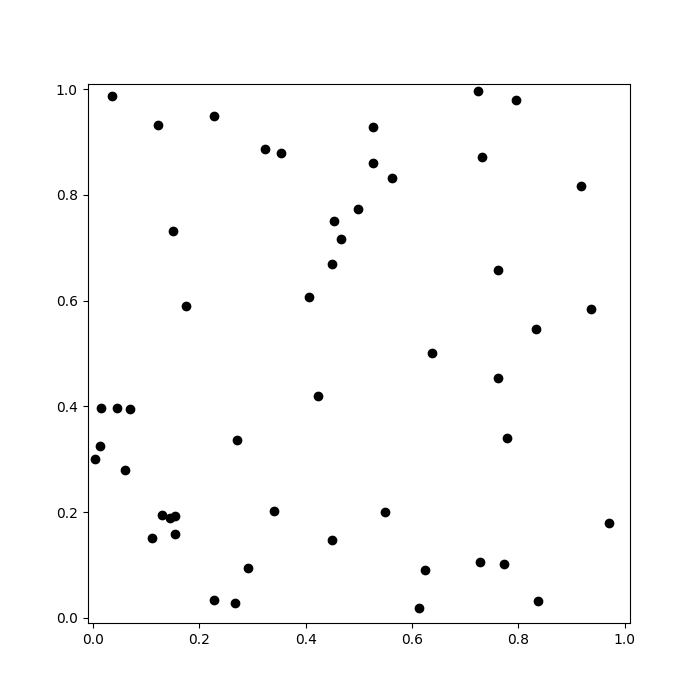
\includegraphics[width=0.33\textwidth]{../Simulation/TSPPictures/ex0.png}
    }
    \subfloat[Divide in $M$ stripes]{\label{TSP:pic0.2}
        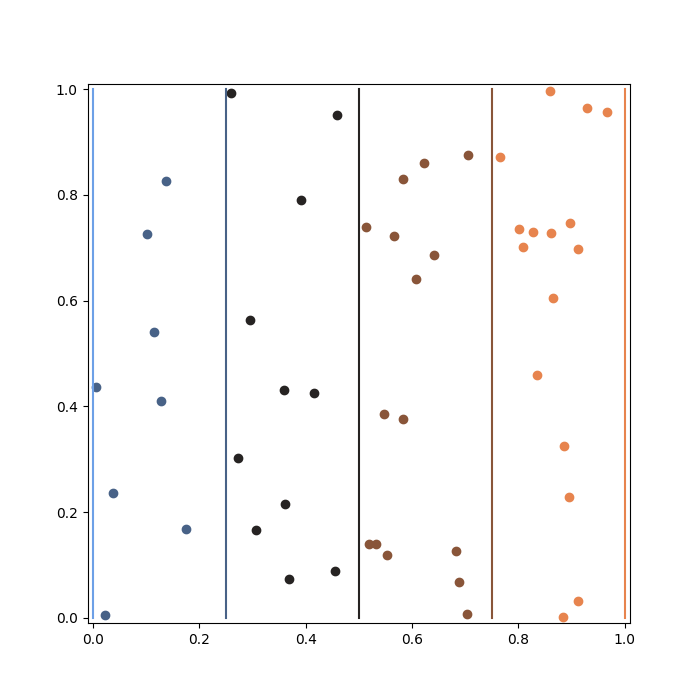
\includegraphics[width=0.33\textwidth]{../Simulation/TSPPictures/ex1.png}
    }
    \subfloat[Join points vertically]{\label{TSP:pic0.3}
        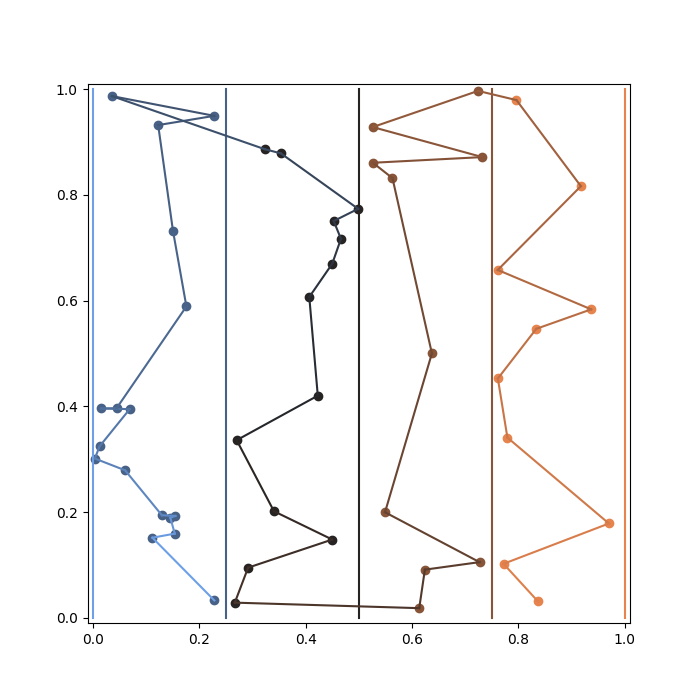
\includegraphics[width=0.33\textwidth]{../Simulation/TSPPictures/ex2.png}
    }
\end{figure}

In the reference~\cite{gzyl1990physicist} the authors assert that by choosing a number of stripes $M^* = \floor{0.58 N^{1/2}}$, one can achieve the best result in comparison to the real TSP solution. If $t_N$ is the TSP solution distance for our sample and $d_N$ is the algorithm's answer with the optimal $M^*$, then the error is asymptotically:
\[  \frac{d_N-t_N}{t_N} \approx 0.23.\] 

The result that we are going to prove is that $d_N$ converges with an exponential rate to its mean. To prove our point, we are going to modify the algorithm's trajectory as it follows. Let $e_N$ be trajectory distance that for any empty stripe in the plane we sum the length of its diagonal $\sqrt{L^2+ L^2/M^2}$ and then it skips the empty stripe. When there are no empty stripes $e_N = d_N$ and the probability that any given stripe is empty converges exponentially to 0:
\[ \begin{array}{rl}
    {(1- 1/M)}^N & = {(1- 0.58^{-1} N^{-1/2})}^N\\[1em]
    & = {\left({(1- 1/M)}^{M}\right)}^{0.58^{-1} N^{1/2}}\\[1em]
    &  \sim \exp(-0.58^{-1} N^{1/2}).
\end{array} \] 


Let $\A_i := \sigma\{X_1,\ldots,X_i\}$ be the sigma algebra corresponding to revealing the first $i$ points, $\A_0 = \{\emptyset, {[0,L]}^2\}$. The expected value of the trajectory $e_N$ given that we only know the positions of the first $i$ points in the sample is $\E (e_N | \A_i)$. Define
\[ Z_i = \E (e_N | \A_i) - \E (e_N | \A_{i-1}),  \]  
As the difference of this expectations when we reveal 1 more point. Note that since
\[ \E(Z_i | \A_i) =  \E (e_N | \A_i, \A_i) - \E (e_N | \A_{i-1}, A_i) = \E (e_N | \A_i) - \E (e_N | \A_i) = 0,\] 
The $Z_i's$ form a vertex exposure martingale sequence.

\begin{figure}[h]\label{TSP:pic1}
    \subfloat[$i = 0$]{\label{TSP:pic1.1}
        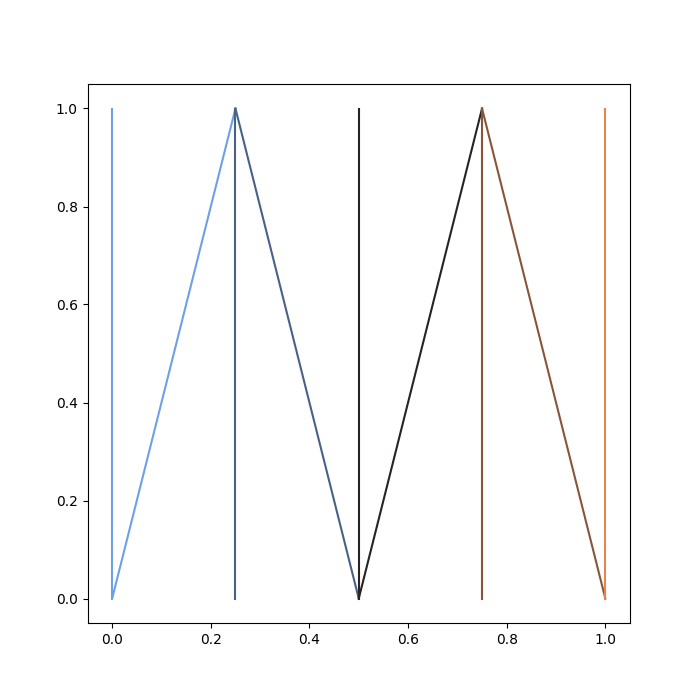
\includegraphics[width=0.25\textwidth]{../Simulation/TSPPictures/pic0.png}
    }
    \subfloat[$i = 1$]{\label{TSP:pic1.2}
        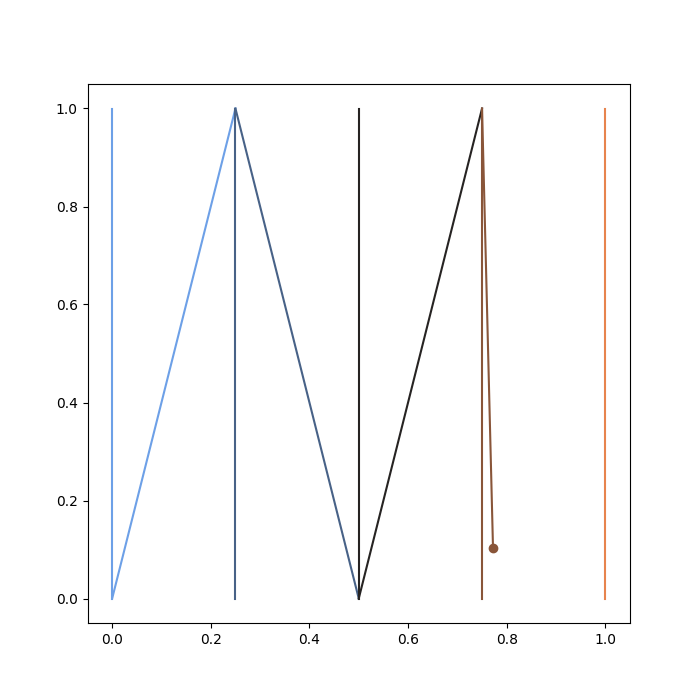
\includegraphics[width=0.25\textwidth]{../Simulation/TSPPictures/pic1.png}
    }
    \subfloat[$i = 2$]{\label{TSP:pic1.3}
        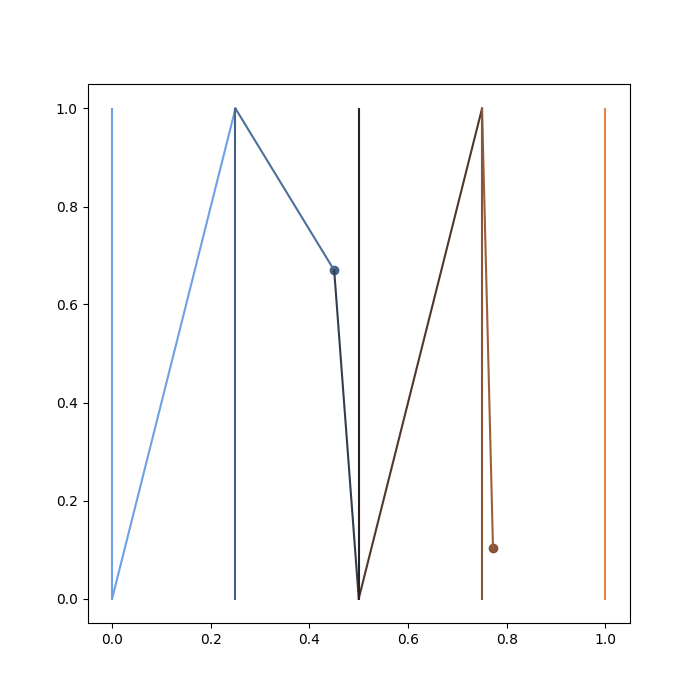
\includegraphics[width=0.25\textwidth]{../Simulation/TSPPictures/pic2.png}
    }
    \subfloat[$i = 4$]{\label{TSP:pic1.4}
        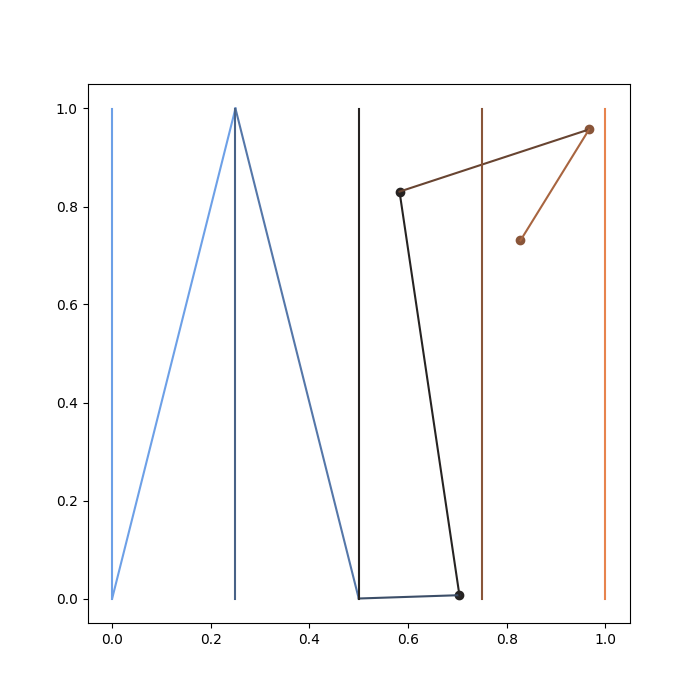
\includegraphics[width=0.25\textwidth]{../Simulation/TSPPictures/pic3.png}
    }

    \subfloat[$i = 7$]{\label{TSP:pic1.5}
        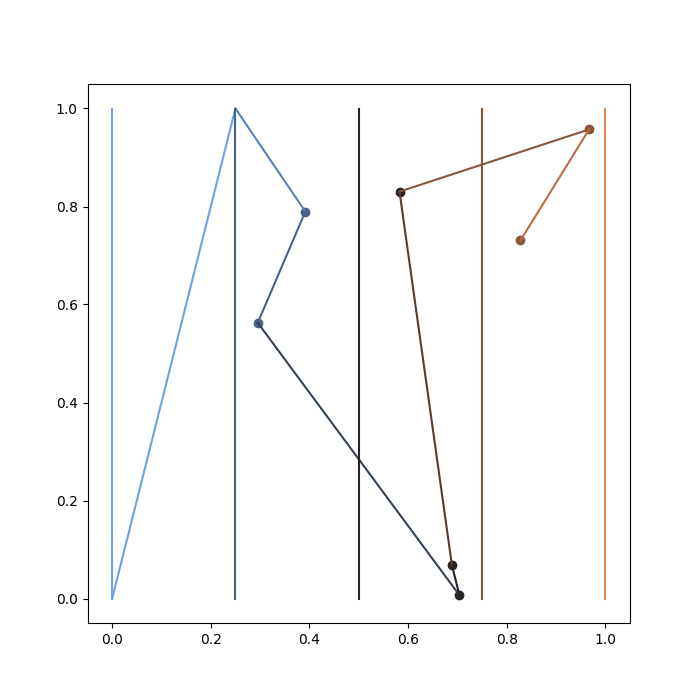
\includegraphics[width=0.25\textwidth]{../Simulation/TSPPictures/pic4.png}
    }
    \subfloat[$i = {12}$]{\label{TSP:pic1.6}
        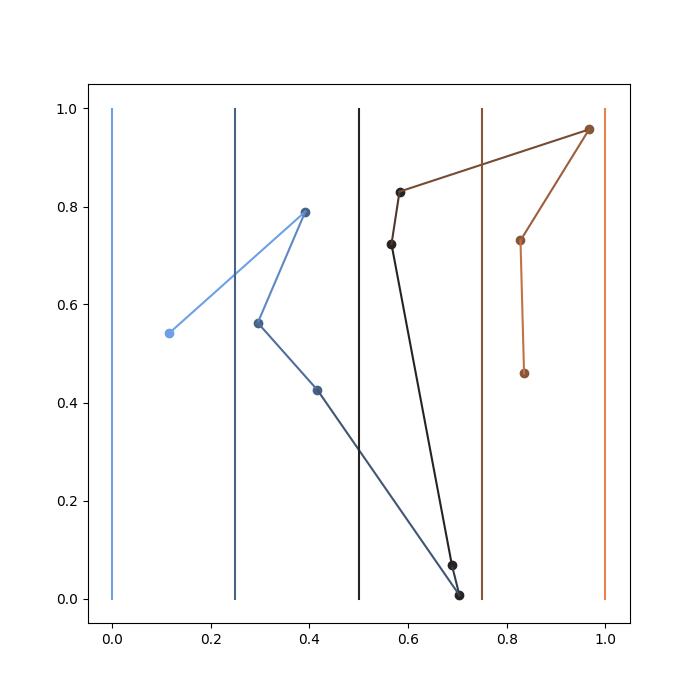
\includegraphics[width=0.25\textwidth]{../Simulation/TSPPictures/pic5.png}
    }
    \subfloat[$i = {18}$]{\label{TSP:pic1.7}
        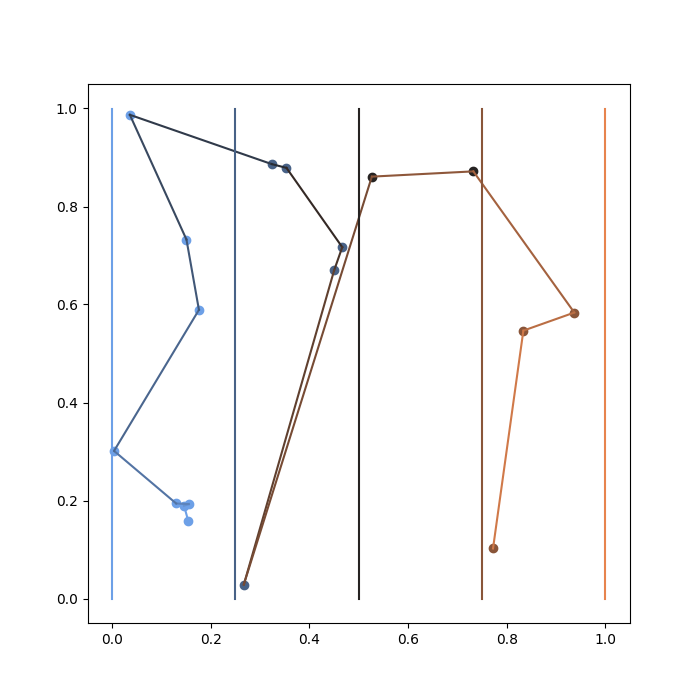
\includegraphics[width=0.25\textwidth]{../Simulation/TSPPictures/pic6.png}
    }
    \subfloat[$i = N = 50$]{\label{TSP:pic1.8}
        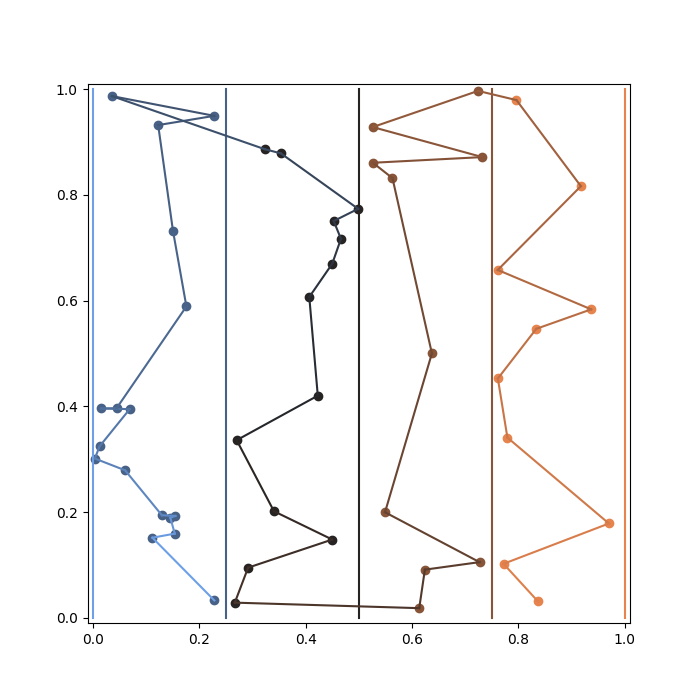
\includegraphics[width=0.25\textwidth]{../Simulation/TSPPictures/ex2.png}
    }
    \caption{Evolution of the Martingale}
\end{figure}

Define $e_N^{[i]}$ as the distance of the trajectory when we remove the $i$-th point from the sample. Intuitively from the figure above and the triangle inequality, we can obtain
\[ e_N^{[i]} \leq e_N \leq e_N + 2 L/M, \]
meaning that revealing one point cannot increase more than 2 widths the distance of the trajectory. Thus,
\[ \|Z_i\|_\infty = \sup_{X_1,\ldots, X_N} \|\E (e_N | \A_i) - \E (e_N | \A_{i-1})\| \leq 2L/M. \]

On the other hand, by telescopic sums we obtain that 
\[  e_N - E e_N = \E (e_N | \A_N) - \E (e_N | \A_{0}) = \sum_{i = 1}^{N} Z_i.\]
Therefore, by the Azuma-Hoeffding inequality,
\[ \P \{ |e_N - E e_N| > t \} \leq 2\exp\left(\frac{-t^2}{2}\sum_{i = 1}^{N} \|Z_i\|_{\infty}^2 \right). \] 
Finally,
\[ \sum_{i = 1}^{N} \|Z_i\|_{\infty}^2 \leq \frac{4NL^2}{M^2}, \]
which implies that
\[\P \{ |e_N - E e_N| > t \} \leq 2\exp\left(\frac{-t^2}{2}\sum_{i = 1}^{N} \frac{4NL^2}{M^2} \right) \sim e^{-t^{2} K N}, \] 
for some $K\in \R^+$.